\section{ADWIN}
\label{sec:ADWIN}
ADWIN należy do grupy algorytmów opartych na koncepcji przesuwnego okna (\textit{sliding window}).
Okno jest zbiorem badanych rekordów o najczęściej jawnie wcześniej zdefiniowanym rozmiarze (rys. \ref{fig:SlidingWindowInit})
do którego wkładane są najnowsze próbki, starsze natomiast są usuwane (rys. \ref{fig:SlidingWindowMove}).
\begin{figure}[htbp]
\centering
	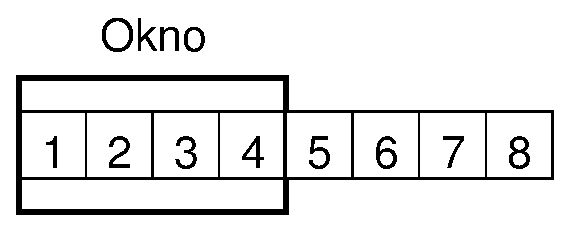
\includegraphics[width=0.5\textwidth]{img/slidingWindowInit}
	\caption{Przesuwne okno - początek}
  \label{fig:SlidingWindowInit}
\end{figure}
\begin{figure}[htbp]
\centering
	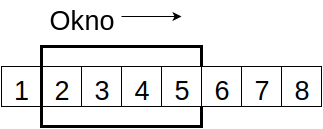
\includegraphics[width=0.5\textwidth]{img/slidingWindowMove}
	\caption{Przesuwne okno - przesuwanie}
  \label{fig:SlidingWindowMove}
\end{figure}
Na podstawie zawartości okna algorytmy mogą:
\begin{itemize}
  \item sprawdzić czy nie zaszła zmiana,
  \item przebudować, zaktualizować model.
\end{itemize}
Dlatego wielkość okna ma znaczenie.
Im jest dłuższe tym algorytmy zachowują się stabilniej w spokojnych okresach,
natomiast im krótsze tym szybciej reagują na zmiany.

Algorytm ADWIN (\textit{ADaptive WINdow}) zaproponowany przez Bifeta (Bifet i in., 2011)
wykorzystuje okno, jednak jego rozmiar jest dynamiczny,
tj. nie ma ustalonego wymiaru i zmienia się w czasie, w zależności od procesowanych danych.

Głównym elementem algorytmu jest przesuwne okno $W$,
którego zawartością są aktualne rekordy $x_{i}$.
W raz z pojawieniem się nowych próbek wewnątrz okna
sprawdzane jest czy wszystkie dostatecznie duże pod-okna nie różnią się względem siebie za bardzo.
Jeśli są różniące się pod-okna to znaczy,
że nastąpiła zmiana. Na koniec kasowane jest starsze pod-okno.
Minimalna wielkość pod-okna i sposób ich porównania zależą od wybranego testu statystycznego
na zgodność rozkładów pod-okien.
\subsection{Testy rozkładu - średnia, wariancja}
\label{sub:TestsMeanAndVar}
Najprostszym sposobem na sprawdzenie czy dwa pod-okna nie różnią się od siebie
jest sprawdzenie czy ich średnie nie różnią się od siebie.
Można to zapisać
$$ | \hat{\mu}_{W_{0}} - \hat{\mu}_{W_{1}} | < \varepsilon, $$
gdzie $W_{0}$ i $W_{1}$ to pod-okna, a $\varepsilon$ to wartość progowa.

Gdy $n_{0}$ to rozmiar $W_{0}$,
a $n_{1}$ to rozmiar $W_{1}$ cały test można zapisać (Bifet i in., 2011)
$$n = n_{0} + n_{1}$$
$$q^\prime = \frac{q}{n}$$
$$m=\frac{1}{\frac{1}{n_0}+\frac{1}{n_1}}$$
$$\varepsilon = \sqrt{\frac{2}{m} \sigma^{2}_{W} \mbox{ln}\frac{2}{q^\prime}} + \frac{2}{3m} + \mbox{ln}\frac{2}{q^\prime},$$
gdzie $\sigma^{2}_{W}$ to wariancja całego okna $W$,
a $q$ to poziom istotności testu.
\subsection{Testy rozkładu - stosunek gęstości}
\label{sub:TestDensityRatio}
